% si-polygraph.tex

%%%%%%%%%%%%%%%%%%%%
\begin{frame}{Dependency Graph-based Characterization of SI}
  \begin{center}
		\only<4>{
			\red{\it Suppose that $T_{A} \rel{\WW} T_{B}$}
		}
		\only<5>{
			$T_{0} \rel{\WR} T_{A} \land T_{0} \rel{\WW} T_{B}
			  \implies T_{A} \rel{\RW} T_{B}$
		}
		\only<6>{
			$T_{0} \rel{\WR} T_{B} \land T_{0} \rel{\WW} T_{A}
			  \implies T_{A} \rel{\RW} T_{A}$
		}
		\only<7->{
			\red{$\boxed{\text{\it Suppose that}\;\; T_{A} \rel{\WW} T_{B}}$}
		}

		\vspace{0.20cm}
		{% banking-lost-update-dep-tikz.tex

\begin{tikzpicture}[
  node distance = 0.8cm and 2.0cm,
  wr/.style = {->, thick},
  ww/.style = {->, thick, dashed, red},
  rw/.style = {->, thick, dotted, blue},
  txn/.style = {draw, inner sep = 3pt, align = center}]

  \node[txn, label = above : $T_{0}$] (t) {$\writeevent(\acct, 0)$};

  \node[txn, label = above : $T_{A}$, above right = of t] (t-alice)
    {$\readevent(\acct, 0)$ \\[2pt] $\writeevent(\acct, 50)$};
  \node[txn, label = below : $T_{B}$, below right = of t] (t-bob)
    {$\readevent(\acct, 0)$ \\[2pt] $\writeevent(\acct, 25)$};

  \node[txn, label = above : $T'_{A}$, right = 6.0cm of t] (t-alice-read) {$\readevent(\acct, 25)$};

  \uncover<2->{
    \draw[wr, sloped] (t) to node[below]{$\WR$} (t-alice.west);
    \draw[wr, sloped] (t) to node[above]{$\WR$} (t-bob.west);
    \draw[wr, sloped] (t-bob.east) to node[below]{$\WR$} (t-alice-read.south);
  }

  \uncover<3->{
    \draw[ww, bend left, sloped] (t) to node[above]{$\WW$} (t-alice);
    \draw[ww, bend right, sloped] (t) to node[below]{$\WW$} (t-bob);
  }
  \uncover<4->{
    \draw[ww] (t-alice) to node[]{$\WW$} (t-bob);
  }

  \uncover<5->{
    \draw[rw, bend right = 60] (t-alice.-145) to node[]{$\RW$} (t-alice.-145 |- t-bob.north);
  }
  \uncover<6->{
    \draw[rw, bend right = 60] (t-bob.35) to node[]{$\RW$} (t-bob.35 |- t-alice.south);
  }
\end{tikzpicture}}
		\vspace{0.20cm}

		\only<2>{
			$\WR$: ``write-read'' dependency capturing the ``read-from'' relation
		}
		\only<3-4>{
			$\WW$: ``write-write'' dependency capturing the version order
		}
		\only<5-6>{
			$\RW$: ``read-write'' dependency capturing the overwritten relation
		}
		\only<7>{
			undesired cycle: $T_{A} \rel{\WW} T_{B} \rel{\RW} T_{A}$
		}
  \end{center}
\end{frame}
%%%%%%%%%%%%%%%%%%%%

%%%%%%%%%%%%%%%%%%%%
\begin{frame}{Dependency Graph-based Characterization of SI}
	\begin{center}
		\uncover<2->{
			\red{$\boxed{\text{\it Suppose that}\;\; T_{B} \rel{\WW} T_{A}}$}
		}

		\vspace{0.20cm}
		{% banking-lost-update-depgraph-ww-tbta-tikz.tex

\begin{tikzpicture}[
  node distance = 0.8cm and 2.0cm,
  wr/.style = {->, thick},
  ww/.style = {->, thick, dashed, red},
  rw/.style = {->, thick, dotted, blue},
  txn/.style = {draw, inner sep = 3pt, align = center}]

  \node[txn, label = above : $T_{0}$] (t) {$\writeevent(\acct, 0)$};

  \node[txn, label = above : $T_{A}$, above right = of t] (t-alice)
    {$\readevent(\acct, 0)$ \\[2pt] $\writeevent(\acct, 50)$};
  \node[txn, label = below : $T_{B}$, below right = of t] (t-bob)
    {$\readevent(\acct, 0)$ \\[2pt] $\writeevent(\acct, 25)$};

  \node[txn, label = above : $T'_{A}$, right = 6.0cm of t] (t-alice-read) {$\readevent(\acct, 25)$};

  \draw[wr, sloped] (t) to node[below]{$\WR$} (t-alice.west);
  \draw[wr, sloped] (t) to node[above]{$\WR$} (t-bob.west);
  \draw[wr, sloped] (t-bob.east) to node[below]{$\WR$} (t-alice-read.south);

  \draw[ww, bend left, sloped] (t) to node[above]{$\WW$} (t-alice);
  \draw[ww, bend right, sloped] (t) to node[below]{$\WW$} (t-bob);
  \uncover<2->{
  \draw[ww] (t-bob) to node[]{$\WW$} (t-alice);
  }

  \draw[rw, bend right = 60] (t-alice.-145) to node[]{$\RW$} (t-alice.-145 |- t-bob.north);
  \draw[rw, bend right = 60] (t-bob.35) to node[]{$\RW$} (t-bob.35 |- t-alice.south);

  \uncover<3->{
  \draw[rw] (t-alice-read.north) to node[sloped, above]{$\RW$} (t-alice.east);
  }
\end{tikzpicture}}
		\vspace{0.20cm}

		\uncover<5>{
			undesired cycle: $T_{B} \rel{\WW} T_{A} \rel{\RW} T_{B}$
		}
	\end{center}
\end{frame}
%%%%%%%%%%%%%%%%%%%%

%%%%%%%%%%%%%%%%%%%%
\begin{frame}{Dependency Graph-based Characterization of SI}
  \begin{center}
		We have considered both bases $T_{A} \rel{\WW} T_{B}$
		and $T_{B} \rel{\WW} T_{A}$.

		\vspace{0.20cm}
		\fig{width = 0.65\textwidth}{figs/banking-lost-update-wr}
		\vspace{0.20cm}

		Either case leads to an undesired cycle. \\[2pt]
		Therefore, it does not satisfy SI.
  \end{center}
\end{frame}
%%%%%%%%%%%%%%%%%%%%

%%%%%%%%%%%%%%%%%%%%
\begin{frame}{Dependency Graph-based Characterization of SI}
  \begin{theorem}[Theorem 4.1 of~\ncite{AnalysingSI:JACM2018}]
		Informally, a history satisfies SI if only if \\[3pt]
		\red{there exists} a dependency graph for it that contains \\[3pt]
		only cycles (if any) with \blue{at least two adjacent $\RW$} edges.
	\end{theorem}
\end{frame}
%%%%%%%%%%%%%%%%%%%%

%%%%%%%%%%%%%%%%%%%%
\begin{frame}{Dependency Graph-based Characterization of SI}
	\begin{columns}
		\column{0.50\textwidth}
			{\fig{width = 1.00\textwidth}{figs/banking-lost-update-depgraph}}
		\column{0.50\textwidth}
			{\fig{width = 1.00\textwidth}{figs/banking-lost-update-depgraph}}
	\end{columns}

	\vspace{0.30cm}
	\begin{center}
		Every possible dependency graph contains
		an undesired \raisebox{-1.0ex}{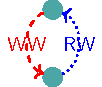
\includegraphics[scale = 0.50]{figs/ww-rw-cycle}} cycle.
	\end{center}
\end{frame}
%%%%%%%%%%%%%%%%%%%%

%%%%%%%%%%%%%%%%%%%%
\begin{frame}{Dependency Graph-based Characterization of SI}
  \begin{theorem}[Theorem 4.1 of~\ncite{AnalysingSI:JACM2018}]
		For a history \emph{$\H = (\T, \SO)$},
		\vspace{-0.30cm}
		\begin{align*}
			\H \models \si & \iff \H \models \intaxiom \;\land \\
				&\red{\exists}\; \WR, \WW, \RW.\; \G = (\H, \WR, \WW, \RW) \;\land \\
				&\quad (\blue{((\SO_{\G} \cup \WR_{\G} \cup \WW_{\G}) \comp \RW_{\G}?)} \text{\it\; is acyclic}).
		\end{align*}
  \end{theorem}

	\begin{center}
		\resizebox{0.60\textwidth}{!}{% banking-lost-update-dep-theorem-tikz.tex

\begin{tikzpicture}[
  node distance = 0.8cm and 2.0cm,
  wr/.style = {->, thick},
  ww/.style = {->, thick, dashed, red},
  rw/.style = {->, thick, dotted, blue},
  txn/.style = {draw, inner sep = 3pt, align = center},
  comp/.style = {->, ultra thick, purple, loosely dash dot}]

  \node[txn, label = above : $T_{0}$] (t) {$\writeevent(\acct, 0)$};

  \node[txn, label = above : $T_{A}$, above right = of t] (t-alice)
    {$\readevent(\acct, 0)$ \\[2pt] $\writeevent(\acct, 50)$};
  \node[txn, label = below : $T_{B}$, below right = of t] (t-bob)
    {$\readevent(\acct, 0)$ \\[2pt] $\writeevent(\acct, 25)$};

  \node[txn, label = above : $T'_{A}$, right = 6.0cm of t] (t-alice-read) {$\readevent(\acct, 25)$};

  \draw[wr, sloped] (t) to node[below]{$\WR$} (t-alice.west);
  \draw[wr, sloped] (t) to node[above]{$\WR$} (t-bob.west);
  \draw[wr, sloped] (t-bob.east) to node[below]{$\WR$} (t-alice-read.south);

  \draw[ww, bend left, sloped] (t) to node[above]{$\WW$} (t-alice);
  \draw[ww, bend right, sloped] (t) to node[below]{$\WW$} (t-bob);
  \draw[ww] (t-alice) to node[]{$\WW$} (t-bob);

  \uncover<1-2>{
  \draw[rw, bend right = 60] (t-alice.-145) to node[]{$\RW$} (t-alice.-145 |- t-bob.north);
  \draw[rw, bend right = 60] (t-bob.35) to node[]{$\RW$} (t-bob.35 |- t-alice.south);
  }

  \uncover<2->{
  \draw[comp, bend left = 30] (t.north west) to (t-alice.north west);
  }
  \uncover<2->{
  \draw[comp, bend right = 30] (t.south west) to (t-bob.south west);
  }
  \uncover<2->{
  \draw[comp] (t-alice.south east) to [out = -30, in = 30, looseness = 4] (t-alice.north east);
  }
\end{tikzpicture}}
	\end{center}
\end{frame}
%%%%%%%%%%%%%%%%%%%%

%%%%%%%%%%%%%%%%%%%%
\begin{frame}{Dependency Graph-based Characterization of SI}
  \begin{center}
		\red{$\mathcal{Q}:$ How to capture and resolve all {possible} $\WW$ dependencies?}

		\vspace{0.50cm}
		\begin{columns}
			\column{0.50\textwidth}
				\fig{width = 1.00\textwidth}{figs/banking-lost-update-depgraph}
			\column{0.50\textwidth}
				\fig{width = 1.00\textwidth}{figs/banking-lost-update-depgraph-ww-tbta}
		\end{columns}

		\pause
		\vspace{0.80cm}
		\blue{$\mathcal{A}:$ encode them into SAT formulas based on \\[2pt]
		  (generalized) polygraphs and solve them using SAT solvers.}
  \end{center}
\end{frame}
%%%%%%%%%%%%%%%%%%%%

%%%%%%%%%%%%%%%%%%%%
\begin{frame}{Polygraphs: A Family of Dependency Graphs}
	\begin{center}
		Consider the two cases of $\WW$ dependencies between $T_{A}$ and $T_{B}$.
	\end{center}

	\begin{columns}[c]
		\column{0.50\textwidth}
			\fig{width = 0.80\textwidth}{figs/banking-lost-update-depgraph}
		\column{0.50\textwidth}
			\fig{width = 0.80\textwidth}{figs/banking-lost-update-depgraph-ww-tbta}
	\end{columns}

	\begin{center}
		\pause
		\fig{width = 0.40\textwidth}{figs/banking-lost-update-polygraph}
		generalized polygraph:

		\pause
		\vspace{-0.30cm}
		\[
			\tuple{\teal{\eithervar} \triangleq \set{T_{A} \rel{\WW} T_{B}},
				\teal{\orvar} \triangleq \set{T_{B} \rel{\WW} T_{A}, T_{A}' \rel{\RW} T_{A}}}
		\]
	\end{center}
\end{frame}
%%%%%%%%%%%%%%%%%%%%

%%%%%%%%%%%%%%%%%%%%
\begin{frame}{\polysi: Pruning before Encoding (the $\WW$ case)}
	\begin{columns}
		\column{0.40\textwidth}
			\fig{width = 0.70\textwidth}{figs/pruning-ww-case}
		\column{0.60\textwidth}
		  \resizebox{1.00\textwidth}{!}{% banking-lost-update-polygraph-pruning-ww-tikz.tex

\begin{tikzpicture}[
  node distance = 0.8cm and 2.0cm,
  wr/.style = {->, thick},
  ww/.style = {->, thick, dashed, red},
  rw/.style = {->, thick, dotted, blue},
  txn/.style = {draw, inner sep = 3pt, align = center}]

  \node[txn, label = above : $T_{0}$] (t) {$\writeevent(\acct, 0)$};

  \node[txn, label = above : $T_{A}$, above right = of t] (t-alice)
    {$\readevent(\acct, 0)$ \\[2pt] $\writeevent(\acct, 50)$};
  \node[txn, label = below : $T_{B}$, below right = of t] (t-bob)
    {$\readevent(\acct, 0)$ \\[2pt] $\writeevent(\acct, 25)$};

  \node[txn, label = above : $T'_{A}$, right = 6.0cm of t] (t-alice-read) {$\readevent(\acct, 25)$};

  \draw[wr, sloped] (t) to node[below]{$\WR$} (t-alice.west);
  \draw[wr, sloped] (t) to node[above]{$\WR$} (t-bob.west);
  \draw[wr, sloped] (t-bob.east) to node[below]{$\WR$} (t-alice-read.south);

  \draw[ww, bend left, sloped] (t) to
    node[above]{$\WW$}
    node[above = -0.60cm, scale = 2]{\yes}
    (t-alice);
  \draw[rw, bend right = 60] (t-bob.35) to
    node[]{$\RW$}
    node[scale = 2]{\yes}
    (t-bob.35 |- t-alice.south);

  \uncover<2->{
  \draw[ww, bend left, sloped] (t-alice) to
    node[above]{$\WW$}
    node[above = -0.80cm, scale = 2]{\no}
    (t.east);
  }
\end{tikzpicture}}
	\end{columns}

	\vspace{0.30cm}
  \begin{center}
		\uncover<2->{
			$T_{A} \rel{\WW} T_{0}$ can be pruned due to the
			$T_{A} \rel{\WW} T_{0} \rel{\WR} T_{A}$ cycle.
		}
  \end{center}
\end{frame}
%%%%%%%%%%%%%%%%%%%%

%%%%%%%%%%%%%%%%%%%%
\begin{frame}{\polysi: Pruning before Encoding (the $\WW$ case)}
	\begin{columns}
		\column{0.40\textwidth}
			\fig{width = 0.60\textwidth}{figs/pruning-ww-case}
		\column{0.60\textwidth}
			\resizebox{1.00\textwidth}{!}{% banking-lost-update-polygraph-pruning-ww-tatb-tikz.tex

\begin{tikzpicture}[
  node distance = 0.8cm and 2.0cm,
  wr/.style = {->, thick},
  ww/.style = {->, thick, dashed, red},
  rw/.style = {->, thick, dotted, blue},
  txn/.style = {draw, inner sep = 3pt, align = center}]

  \node[txn, label = above : $T_{0}$] (t) {$\writeevent(\acct, 0)$};

  \node[txn, label = above : $T_{A}$, above right = of t] (t-alice)
    {$\readevent(\acct, 0)$ \\[2pt] $\writeevent(\acct, 50)$};
  \node[txn, label = below : $T_{B}$, below right = of t] (t-bob)
    {$\readevent(\acct, 0)$ \\[2pt] $\writeevent(\acct, 25)$};

  \node[txn, label = above : $T'_{A}$, right = 6.0cm of t] (t-alice-read) {$\readevent(\acct, 25)$};

  \draw[wr, sloped] (t) to node[below]{$\WR$} (t-alice.west);
  \draw[wr, sloped] (t) to node[above]{$\WR$} (t-bob.west);
  \draw[wr, sloped] (t-bob.east) to node[below]{$\WR$} (t-alice-read.south);

  \draw[ww, bend left, sloped] (t) to
    node[above]{$\WW$}
    node[scale = 2]{\yes}
    (t-alice);
  \draw[ww, bend right, sloped] (t) to
    node[below]{$\WW$}
    node[scale = 2]{\yes}
    (t-bob);
  \uncover<3->{
  \draw[ww] (t-bob.45) to
    node[]{$\WW$}
    node[below = 0.30cm, anchor = center, scale = 2]{\no}
    (t-bob.45 |- t-alice.south);
  }
  \uncover<2->{
    \draw[ww] (t-alice.-135) to
      node[]{$\WW$}
      node[below = 0.30cm, anchor = center, scale = 2]{\no}
      (t-alice.-135 |- t-bob.north);
  }

  \draw[rw, bend right = 60] (t-alice.-145) to
    node[]{$\RW$}
    node[scale = 2]{\yes}
    (t-alice.-145 |- t-bob.north);
  \draw[rw, bend right = 60] (t-bob.35) to
    node[]{$\RW$}
    node[scale = 2]{\yes}
    (t-bob.35 |- t-alice.south);

  \uncover<3->{
  \draw[rw] (t-alice-read.north) to
    node[sloped, above]{$\RW$}
    node[right, scale = 2]{\no}
    (t-alice.east);
  }
\end{tikzpicture}}
	\end{columns}

	\vspace{0.30cm}
  \begin{center}
		\uncover<2->{
		$T_{A} \rel{\WW} T_{B}$ is pruned due to the $T_{A} \rel{\WW} T_{B} \rel{\RW} T_{A}$ cycle. \\[2pt]
		}
		\uncover<3->{
		$T_{B} \rel{\WW} T_{A}$ is pruned due to the $T_{B} \rel{\WW} T_{A} \rel{\RW} T_{B}$ cycle. \\[8pt]
		}
		\uncover<4->{
		\red{Therefore, we are sure that the history does {\it not} satisfy SI.}
		}
  \end{center}
\end{frame}
%%%%%%%%%%%%%%%%%%%%

%%%%%%%%%%%%%%%%%%%%
\begin{frame}{\polysi: Pruning before Encoding (the $\RW$ case)}
  \begin{center}
		\resizebox{0.40\textwidth}{!}{% pruning-rw-case-tikz.tex

\begin{tikzpicture}[vertex/.style = {circle, draw, minimum size = 30pt},
  edge/.style = {->, thick},
  path/.style = {->, thick, decorate, decoration = snake}]

  \node[vertex] (from) {$\mathit{from}$};
  \node[vertex, right = 2.0cm of from] (to) {$\mathit{to}$};
  \draw[edge, blue] (from) to node[above, blue]{\textsf{RW}} (to);

  \uncover<2->{
  \node[vertex, below = 2.5cm of from, fill = yellow!50] (prec) {$\mathit{prec}$};

  \draw[edge] (prec) to[sloped] node[above, purple]{{\it not} \textsf{RW} edge} (from);
  \draw[path] (to) to[bend left = 70, sloped]
    node[above]{no \textsf{RW} edges}
    (prec);
  }

  \uncover<3->{
  \draw[edge, dashed] (prec) to[sloped]
    % node[above]{in $\knowninducedgraph$}
    (to);
  }
\end{tikzpicture}}
  \end{center}

	\uncover<3->{
  \begin{theorem}[Theorem 4.1 of~\ncite{AnalysingSI:JACM2018}]
		Informally, a history satisfies SI if only if \\[3pt]
		\red{there exists} a dependency graph for it that contains \\[3pt]
		only cycles (if any) with \blue{at least two adjacent $\RW$} edges.
	\end{theorem}
	}
\end{frame}
%%%%%%%%%%%%%%%%%%%%

%%%%%%%%%%%%%%%%%%%%
\begin{frame}{\textsc{PolySI}: An Illustrating Example of ``Long Fork''}
	\begin{center}
		\resizebox{0.90\textwidth}{!}{% polysi-alg-tikz.tex

\begin{tikzpicture}[
  node distance = 0.8cm and 1.5cm,
  so/.style = {->, thick},
  wr/.style = {->, thick},
  ww/.style = {->, thick, dashed, red},
  rw/.style = {->, thick, dotted, blue},
  txn/.style = {draw, inner sep = 2pt},
  hl/.style = {fill = yellow!50},]

  \uncover<1-17>{
    % t0
    \node[txn, label = left : $T_{0}$, onslide={<7,8,9,11,12,13,15>{hl}}] (t0)
      {$\writeevent(\keyxvar, 0) \; \writeevent(\keyyvar, 0)$};
  }
  \uncover<6-17>{
    % t5
    \node[txn, label = right : $T_{5}$, right = 2.50cm of t0, onslide={<7,8,9,17>{hl}}] (t5)
      {$\writeevent(\keyxvar, 2)$};
    % t0 SO t5
    \draw[so] (t0.east) to node[above, sloped, very near end]{$\SO$} (t5);
  }

  \uncover<2->{
    % t1
    \node[txn, label = above : $T_{1}$, above right = 1.00cm and -1.00cm of t0, onslide={<11,12,13,17>{hl}}] (t1)
      {$\writeevent(\keyxvar, 1)$};
  }
  \uncover<3->{
    % t2
    \node[txn, label = below : $T_{2}$, onslide = <15>{hl}, below right = 1.00cm and -1.00cm of t0] (t2)
      {$\writeevent(\keyyvar, 1)$};
  }

  \uncover<4->{
    \node[txn, right = of t1, label = above : $T_{3}$] (t3)
      {$\readevent(\keyxvar, 1) \; \readevent(\keyyvar, 0)$};
    % t1 WR(x) t3
    \draw[wr] (t1) to node[above]{$\WR(\keyxvar)$} (t3);
  }
  \uncover<4-17>{
    % t0 WR(y) t3
    \draw[wr] (t0.east) to node[below, sloped, very near end]{$\WR(\keyyvar)$} (t3.-20);
  }
  \uncover<5->{
    \node[txn, right = of t2, label = below : $T_{4}$] (t4)
      {$\readevent(\keyxvar, 0) \; \readevent(\keyyvar, 1)$};
    % t2 WR(y) t4
    \draw[wr] (t2) to node[below]{$\WR(\keyyvar)$} (t4);
  }
  \uncover<5-17>{
    % t0 WR(x) t4
    \draw[wr] (t0.east) to node[above, sloped, very near end]{$\WR(\keyxvar)$} (t4.20);
  }

  \uncover<7>{
    % no: t5 WW(x) t0
    \draw[ww, bend right = 20] (t5) to node[above, sloped]{$\WW(\keyxvar)$} (t0);
    \draw[ww, bend right = 20] (t5) to node[above, sloped]{\Large\no} (t0);
  }

  \uncover<8>{
  }

  \uncover<9>{
    % yes: t0 WW(x) t5
    \draw[ww, bend right = 20] (t0) to node[below, sloped]{$\WW(\keyxvar)$} (t5);
    \draw[ww, bend right = 20] (t0) to node[below, sloped]{\Large\yes} (t5);
    % yes: t4 RW(x) t5
    \draw[rw] (t4.160) to node[above = -5pt, sloped]{$\RW(\keyxvar)$}
      node[] {\Large\yes}
      (t5);
  }
  \uncover<10-17>{
    % t0 WW(x) t5
    \draw[ww, bend right = 20] (t0) to node[below, sloped]{$\WW(\keyxvar)$} (t5);
    % t4 RW(x) t5
    \draw[rw] (t4.160) to node[above = -5pt, sloped]{$\RW(\keyxvar)$} (t5);
  }

  \uncover<11>{
    % t1 WW(x) t0
    \draw[ww] (t1) to node[pos = 0.30, below] {$\WW(\keyxvar)$}
      node[pos = 0.40]{\Large\no} (t0);
    % t3 RW(x) t0
    \draw[rw] (t3) to node[pos = 0.40, above, sloped] {$\RW(\keyxvar)$}
      node[pos = 0.40]{\Large\no} (t0.15);
  }

  \uncover<12>{}

  \uncover<13>{
    % t0 WW(x) t1
    \draw[ww] (t0.150) to node[above, sloped] {$\WW(\keyxvar)$}
      node[pos = 0.50]{\Large\yes}
      (t1.west);
    % t4 RW(x) t1
    \draw[rw] (t4.160) to node[near end, above, sloped] {$\RW(\keyxvar)$}
      node[above]{\Large\yes}
      (t1.south);
  }
  \uncover<14-17>{
    % t0 WW(x) t1
    \draw[ww] (t0.150) to node[above, sloped] {$\WW(\keyxvar)$} (t1.west);
  }
  \uncover<14-17>{
    % t4 RW(x) t1
    \draw[rw] (t4.160) to node[near end, above, sloped] {$\RW(\keyxvar)$} (t1.south);
  }

  \uncover<15>{
    % t0 WW(y) t2
    \draw[ww] (t0.-150) to node[above, sloped] {$\WW(\keyyvar)$}
      node[pos = 0.50]{\Large\yes} (t2.west);
    % t3 RW(y) t2
    \draw[rw] (t3) to node[near start, above, sloped] {$\RW(\keyyvar)$}
      node[near start]{\Large\yes} (t2);
  }

  \uncover<16-17>{
    % t0 WW(y) t2
    \draw[ww] (t0.-150) to node[above, sloped] {$\WW(\keyyvar)$} (t2.west);
    % t3 RW(y) t2
    \draw[rw] (t3) to node[near start, above, sloped] {$\RW(\keyyvar)$} (t2);
  }
\end{tikzpicture}}

		\only<6>{
			% A ``long fork'' history with $\SO$ and $\WR$ edges.
			order between $T_{0}$, $T_{1}$, and $T_{5}$ (on $\keyxvar$)
			and between $T_{0}$ and $T_{2}$ (on $\keyyvar$)
		}

		\only<7>{
			The $T_{5} \rel{\WW(\keyxvar)} T_{0}$ case is pruned
			due to $T_{0} \rel{\SO} T_{5} \rel{\WW(\keyxvar)} T_{0}$.
		}

		\only<9>{
			The $T_{0} \rel{\WW(\keyxvar)} T_{5}$ case becomes known.
		}

		\only<11>{
			The $T_{1} \rel{\WW(\keyxvar)} T_{0}$ case is pruned
			due to $T_{3} \rel{\RW(\keyxvar)} T_{0} \rel{\WR(\keyyvar)} T_{3}$.
		}

		\only<13>{
			The $T_{0} \rel{\WW(\keyxvar)} T_{1}$ case becomes known.
		}

		\only<15>{
			The $T_{2} \rel{\WW(\keyyvar)} T_{0}$ case is pruned, \\
			while the $T_{0} \rel{\WW(\keyyvar)} T_{2}$ case becomes known.
		}
		\only<17>{
			The order between $T_{1}$ and $T_{5}$ is still uncertain after pruning.
		}
	\end{center}
\end{frame}
%%%%%%%%%%%%%%%%%%%%

%%%%%%%%%%%%%%%%%%%%
\begin{frame}{\textsc{PolySI}: An Illustrating Example of ``Long Fork''}
	\vspace{-0.50cm}
	\[\tuple{
		\uncover<2->{\purple{\eithervar} = \set{T_{1} \rel{\WW(\keyxvar)} T_{5},
			T_{3} \rel{\RW(\keyxvar)} T_{5}}},
		\uncover<3->{\violet{\orvar} = \set{T_{5} \rel{\WW(\keyxvar)} T_{1}}}
	}\]

	\vspace{-0.30cm}
	\begin{center}
		\resizebox{0.80\textwidth}{!}{% polysi-alg-encoding-tikz.tex

\begin{tikzpicture}[
  node distance = 0.8cm and 1.5cm,
  so/.style = {->, thick},
  wr/.style = {->, thick},
  ww/.style = {->, thick, dashed, red},
  rw/.style = {->, thick, dotted, blue},
  txn/.style = {draw, inner sep = 2pt},
  hl/.style = {fill = yellow!50},]

    % t0
    \node[txn, label = left : $T_{0}$] (t0)
      {$\writeevent(\keyxvar, 0) \; \writeevent(\keyyvar, 0)$};
    % t5
    \node[txn, label = right : $T_{5}$, right = 2.50cm of t0, hl] (t5)
      {$\writeevent(\keyxvar, 2)$};
    % t1
    \node[txn, label = above : $T_{1}$, above right = 1.00cm and -1.00cm of t0, hl] (t1)
      {$\writeevent(\keyxvar, 1)$};
    % t2
    \node[txn, label = below : $T_{2}$, below right = 1.00cm and -1.00cm of t0] (t2)
      {$\writeevent(\keyyvar, 1)$};

    % t3
    \node[txn, right = of t1, label = above : $T_{3}$] (t3)
      {$\readevent(\keyxvar, 1) \; \readevent(\keyyvar, 0)$};
    % t1 WR(x) t3
    \draw[wr] (t1) to node[above]{$\WR(\keyxvar)$} (t3);

    % t4
    \node[txn, right = of t2, label = below : $T_{4}$] (t4)
      {$\readevent(\keyxvar, 0) \; \readevent(\keyyvar, 1)$};

  \uncover<2->{
    % t1 WW(x) t5
    \draw[ww] (t1) to node[above, sloped]{$\WW(\keyxvar)$} (t5.north);
    % t3 RW(x) t5
    \draw[rw] (t3) to node[right]{$\RW(\keyxvar)$} (t5.north);
  }

  \uncover<3->{
    % t5 WW(x) t1
    \draw[ww] (t5.west) to node[below, sloped]{$\WW(\keyxvar)$} (t1.-150);
  }
\end{tikzpicture}}
	\end{center}
	\vspace{-0.50cm}

	\uncover<4->{
		\[
			\purple{(\BV_{1,5} \land \BV_{3,5} \land \lnot \BV_{5,1})} \lor
			\violet{(\BV_{5,1} \land \lnot \BV_{1,5} \land \lnot \BV_{3,5})}
		\]
	}
\end{frame}
%%%%%%%%%%%%%%%%%%%%

%%%%%%%%%%%%%%%%%%%%
\begin{frame}{\textsc{PolySI}: An Illustrating Example of ``Long Fork''}
	\vspace{-0.50cm}
	\uncover<2->{
	\[
		\purple{\boxed{((\SO_{\G} \cup \WR_{\G} \cup \WW_{\G}) \comp \RW_{\G}?)}} \text{\it\; is acyclic}.
	\]
	}

	\vspace{-0.40cm}
  \begin{columns}
		\column{0.50\textwidth}
			\fig{width = 1.00\textwidth}{figs/polysi-alg-final}
		\column{0.50\textwidth}
			\fig{width = 1.00\textwidth}{figs/polysi-alg-encoding}
	\end{columns}

	\uncover<3->{
	\begin{center}
		We need to encode the \purple{``composition ($\comp$)''} of dependency edges.
	\end{center}
	}

	\vspace{0.20cm}
	\uncover<4->{
	\[
		T_{1} \rel{\WR} T_{3} \rel{\RW} T_{2}:\;
		  \BV_{1,2}^{\red{I}} = \BV_{1,3} \land \BV_{3,2} \quad
			(\red{I}\; \text{for the induced graph})
	\]
	}
	\vspace{-0.30cm}
	\uncover<5->{
	\[
		T_{1} \rel{\WR} T_{3} \rel{\RW} T_{5}:\;
		  \BV_{1,5}^{\red{I}} = \BV_{1,3} \land \BV_{3,5} \quad
			(\red{I}\; \text{for the induced graph})
	\]
	}
\end{frame}
%%%%%%%%%%%%%%%%%%%%

%%%%%%%%%%%%%%%%%%%%
\begin{frame}{\textsc{PolySI}: An Illustrating Example of ``Long Fork''}
	\begin{center}
		Feed the SAT formula into the \blue{MonoSAT} solver~\ncite{MonoSAT:AAAI2015}
		optimized for \purple{\it cycle detection}

		\vspace{0.20cm}
		\fig{width = 0.40\textwidth}{figs/sat-solver}
		\vspace{0.20cm}

		Assert that the induced graph $\red{I}$ is acyclic.
	\end{center}
\end{frame}
%%%%%%%%%%%%%%%%%%%%

%%%%%%%%%%%%%%%%%%%%
\begin{frame}{\textsc{PolySI}: An Illustrating Example of ``Long Fork''}
	\begin{center}
		\fig{width = 0.50\textwidth}{figs/polysi-alg-cycle}

		\vspace{0.20cm}
		The undesired cycle for ``long fork'' found by MonoSAT.
	\end{center}
\end{frame}
%%%%%%%%%%%%%%%%%%%%